\documentclass[12pt]{article}
\usepackage[T1]{fontenc}
\usepackage[utf8]{inputenc}
\usepackage{polski}
\usepackage{minted}
\usepackage{geometry}
\usepackage{natbib}
\usepackage{enumitem}
\usepackage{graphicx}
\usepackage{bold-extra}
\usepackage[font=small,labelfont=bf]{caption}
\usepackage{hyperref}
\usepackage{titlesec}
\usepackage{indentfirst}
\hyphenpenalty=10000
\tolerance=1000 \emergencystretch=2em
\titlelabel{\thetitle.\quad}



\setminted[java]{
                frame=lines,
                framesep=2mm,
                fontsize=\scriptsize,
                linenos
                }


\setminted[python]{
                frame=lines,
                framesep=2mm,
                fontsize=\scriptsize,
                linenos
                }

 \geometry{
     left=23mm,
     top=25mm,
     right=23mm
 }


\def\mydate{\leavevmode\hbox{\twodigits\day.\twodigits\month.\the\year}}
\def\twodigits#1{\ifnum#1<10 0\fi\the#1}

\begin{document}
%titlepage
\thispagestyle{empty}
\begin{center}
\begin{minipage}{0.75\linewidth}
    \centering
    
\includegraphics[width=0.45\linewidth]{agh_logo2.png}
    \par
    \vspace{2cm}
    {\bfseries{\scshape{\Huge  Systemy rozproszone}}}
    \par
    \vspace{1.7cm}
    {\scshape{\Large Laboratorium 1}}
    \par
    \vspace{0.8cm}
    {\scshape{\Large Gniazda TCP/UDP}}
    \par
    \vspace{3cm}

    {\scshape{\Large Albert Gierlach}}\par
    \vspace{1cm}

    {\Large \mydate}
\end{minipage}
\end{center}
\clearpage



\section{Zadanie 1}

\begin{minted}{java}
public class JavaUdpServer {
    public static void main(String[] args) {
        System.out.println("JAVA UDP SERVER");

        int portNumber = 9008;
        try (DatagramSocket socket = new DatagramSocket(portNumber)) {
            var receiveBuffer = new byte[1024];

            while (true) {
                Arrays.fill(receiveBuffer, (byte) 0);
                var packet = new DatagramPacket(receiveBuffer, receiveBuffer.length);
                socket.receive(packet);
                var msg = new String(receiveBuffer, 0, packet.getLength());
                System.out.println("received msg: " + msg + " from: " + packet.getAddress());

                var toSend = "JAVA UDP SERVER response";
                System.out.println("Sending: " + toSend);
                socket.send(new DatagramPacket(toSend.getBytes(), toSend.length(), packet.getAddress(), packet.getPort()));
            }
        } catch (Exception e) {
            e.printStackTrace();
        }
    }
}
\end{minted}

\begin{minted}{java}
public class JavaUdpClient {
    public static void main(String[] args) {
        System.out.println("JAVA UDP CLIENT");

        int portNumber = 9008;
        try (DatagramSocket socket = new DatagramSocket()) {
            var address = InetAddress.getByName("localhost");
            var sendBuffer = "Ping Java Udp".getBytes();

            var sendPacket = new DatagramPacket(sendBuffer, sendBuffer.length, address, portNumber);
            socket.send(sendPacket);

            var receiveBuffer = new byte[1024];
            var receivePacket = new DatagramPacket(receiveBuffer, receiveBuffer.length);
            socket.receive(receivePacket);
            var receivedString = new String(receiveBuffer, 0, receivePacket.getLength());
            System.out.println("Received: " + receivedString + " from: " + receivePacket.getAddress());
        } catch (Exception e) {
            e.printStackTrace();
        }
    }
}
\end{minted}

W klasie \emph{JavaUdpServer} została dodana obsługa pobierania adresu nadawcy (metoda \emph{.getAddress()}) oraz wysyłanie odpowiedzi poprzez metodę \emph{.send()} na odpowiedni adres i port (linie 14-18). Klasa klienta została rozszerzona o odbieranie wiadomości od serwera oraz jej wypisanie (linie 13-17).

\begin{center}
\centering
    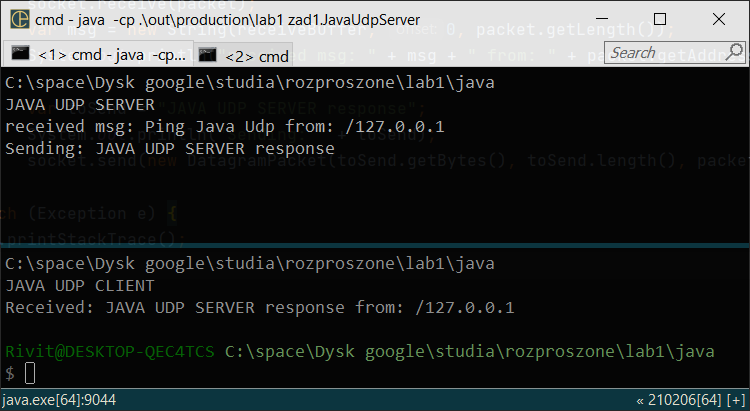
\includegraphics[scale=0.8]{1.png}
    \captionof{figure}{Wynik działania programów}
\end{center}


\section{Zadanie 2}
\begin{minted}{java}
public class JavaUdpServer {
    public static void main(String[] args) {
        System.out.println("JAVA UDP SERVER");

        int portNumber = 9008;
        try (DatagramSocket socket = new DatagramSocket(portNumber)) {
            byte[] receiveBuffer = new byte[1024];

            while(true){
                Arrays.fill(receiveBuffer, (byte) 0);
                var receivePacket = new DatagramPacket(receiveBuffer, receiveBuffer.length);

                socket.receive(receivePacket);
                var msg = new String(receiveBuffer, 0, receivePacket.getLength());
                System.out.println("received msg: " + msg + " from: " + receivePacket.getAddress());
            }
        } catch (Exception e) {
            e.printStackTrace();
        }
    }
}
\end{minted}


\begin{minted}{python}
serverIP = "127.0.0.1"
serverPort = 9008
msg = "żółta gęś"

print('PYTHON UDP CLIENT')
client = socket.socket(socket.AF_INET, socket.SOCK_DGRAM)
client.sendto(bytes(msg, 'utf8'), (serverIP, serverPort))
\end{minted}

Jedyna zmiana jaka została wprowadzona dotyczy programu napisanego w Pythonie. Kodowanie znaków zostało zmienione na UTF-8, aby wiadomość została poprawnie zdekodowana po stronie serwera (linia 7).

\begin{center}
\centering
    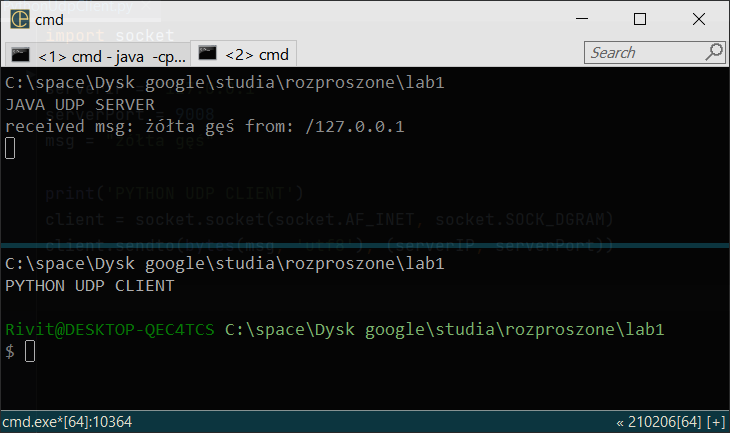
\includegraphics[scale=0.8]{2.png}
    \captionof{figure}{Wynik działania programów}
\end{center}

\section{Zadanie 3}

\begin{minted}{java}
public class JavaUdpServer {
    public static void main(String[] args) {
        System.out.println("JAVA UDP SERVER");

        int portNumber = 9008;
        try (DatagramSocket socket = new DatagramSocket(portNumber)) {
            byte[] receiveBuffer = new byte[1024];

            while(true){
                Arrays.fill(receiveBuffer, (byte) 0);
                var receivePacket = new DatagramPacket(receiveBuffer, receiveBuffer.length);
                socket.receive(receivePacket);

                var num = ByteBuffer.wrap(receiveBuffer).order(ByteOrder.LITTLE_ENDIAN).getInt();
                System.out.println("received number: " + num++);

                var buff = ByteBuffer.allocate(4).order(ByteOrder.LITTLE_ENDIAN).putInt(num).array();
                socket.send(new DatagramPacket(buff, buff.length, receivePacket.getAddress(), receivePacket.getPort()));
            }
        } catch (Exception e) {
            e.printStackTrace();
        }
    }
}
\end{minted}

\newpage
\begin{minted}{python}
serverIP = "127.0.0.1"
serverPort = 9008
msg_bytes = (300).to_bytes(4, byteorder='little')

print('PYTHON UDP CLIENT')
client = socket.socket(socket.AF_INET, socket.SOCK_DGRAM)
client.sendto(msg_bytes, (serverIP, serverPort))

buff, _ = client.recvfrom(1024)
num = int.from_bytes(buff, byteorder='little')
print(f"Received {num}")
\end{minted}

Klasa \emph{JavaUdpServer} została rozszerzona o poprawną obsługę zamiany kolejności bajtów (metoda \emph{.order()}), które są odczytywane z pakietu datagramowego. Następnie zwiększamy otrzymaną liczbę, zamieniamy ją na format little endian i odsyłamy do klienta (linie 14-18). Kod klienta sprowadza się do zakodowania liczby do postaci little endian, wysłania jej oraz oczekiwania na odpowiedź od serwera. 

\begin{center}
\centering
    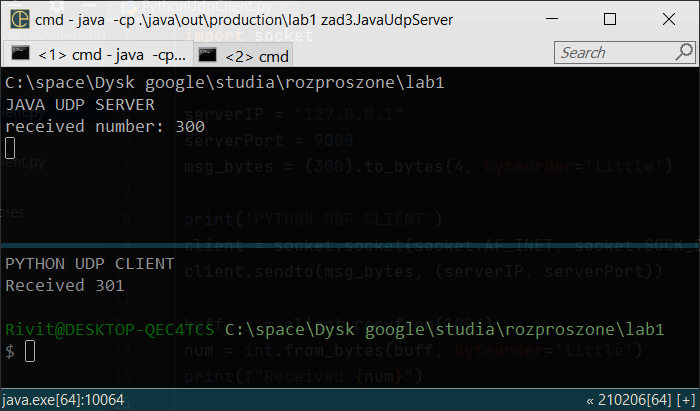
\includegraphics[scale=0.8]{3.png}
    \captionof{figure}{Wynik działania programów}
\end{center}

\newpage
\section{Zadanie 4}

\begin{minted}{java}
public class JavaUdpServer {
    public static void main(String[] args) {
        System.out.println("JAVA UDP SERVER");

        int portNumber = 9008;
        try (DatagramSocket socket = new DatagramSocket(portNumber)) {
            byte[] receiveBuffer = new byte[1024];

            while(true){
                Arrays.fill(receiveBuffer, (byte) 0);
                var receivePacket = new DatagramPacket(receiveBuffer, receiveBuffer.length);
                socket.receive(receivePacket);

                var msg = new String(receiveBuffer, 0, receivePacket.getLength());
                System.out.println("Received: " + msg);
                var response = "";
                if(msg.toLowerCase().contains("python")){
                    response = "Pong Python";
                }else if(msg.toLowerCase().contains("java")){
                    response = "Pong Java";
                }

                socket.send(new DatagramPacket(response.getBytes(), response.length(), receivePacket.getAddress(), receivePacket.getPort()));
            }
        } catch (Exception e) {
            e.printStackTrace();
        }
    }
}
\end{minted}

\begin{minted}{java}
public class JavaUdpClient {
    public static void main(String[] args) {
        System.out.println("JAVA UDP CLIENT");

        int portNumber = 9008;
        try (DatagramSocket socket = new DatagramSocket()) {
            var receiveBuffer = new byte[1024];

            var address = InetAddress.getByName("localhost");
            var sendBuffer = "Ping Java".getBytes();
            var sendPacket = new DatagramPacket(sendBuffer, sendBuffer.length, address, portNumber);
            socket.send(sendPacket);

            var receivePacket = new DatagramPacket(receiveBuffer, receiveBuffer.length);
            socket.receive(receivePacket);
            var receivedString = new String(receiveBuffer, 0, receivePacket.getLength());
            System.out.println("Response: " + receivedString);
        } catch (Exception e) {
            e.printStackTrace();
        }
    }
}
\end{minted}

\newpage
\begin{minted}{python}
serverIP = "127.0.0.1"
serverPort = 9008
msg = "Ping Python"

print('PYTHON UDP CLIENT')
client = socket.socket(socket.AF_INET, socket.SOCK_DGRAM)
client.sendto(bytes(msg, 'utf8'), (serverIP, serverPort))

buff, _ = client.recvfrom(1024)
print(f"Response: {buff.decode()}")
\end{minted}

Server rozpoznaje typ klienta od którego dostał wiadomość poprzez sprawdzenie treści wiadomości (linie 14-23). Jeśli treść wiadomości zawiera słowo "python" to oznacza, że wiadomość przyszła od klienta napisanego w języku Python - analogicznie z językiem Java. Klienci czekają na odpowiedź serwera, a następnie ją wypisują.


\begin{center}
\centering
    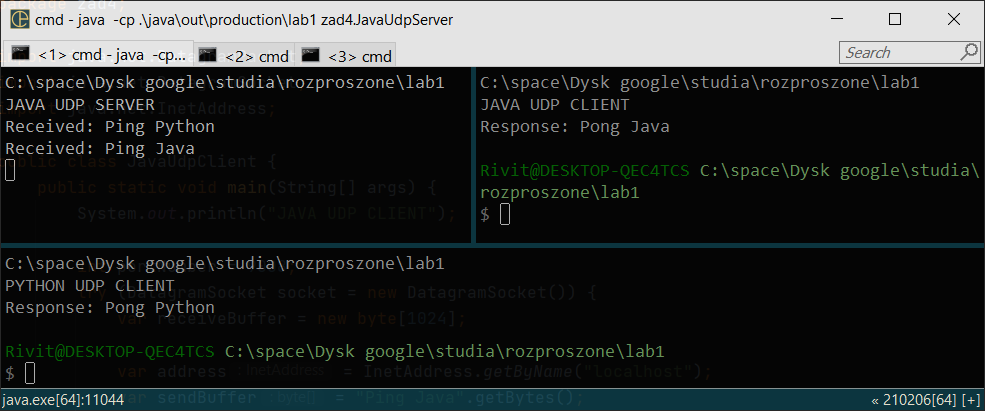
\includegraphics[scale=0.8]{4.png}
    \captionof{figure}{Wynik działania programów}
\end{center}

\end{document}
